\documentclass[5p,twocolumn,10pt,times]{elsarticle}
\usepackage{amsmath}
\usepackage[draft]{hyperref} % added [draft] to avoid compilation issues that happen if a link is split and appears in two pages
%\modulolinenumbers[5]
\addtolength{\textheight}{8mm}
\addtolength{\textwidth}{4mm}
\addtolength{\voffset}{-10mm}
\addtolength{\hoffset}{-3mm}

\bibliographystyle{elsarticle-num-names}


% ACM template
%
%\documentclass[acmtog,anonymous,timestamp,review]{acmart}
%
%\usepackage{booktabs} % For formal tables
%




% My TK added packages and commands

	% for for using hyperref and elsarticle-num-names together in order to get \citeauthor to work
	\makeatletter
	\providecommand{\doi}[1]{%
	  \begingroup
	    \let\bibinfo\@secondoftwo
	    \urlstyle{rm}%
	    \href{http://dx.doi.org/#1}{%
	      doi:\discretionary{}{}{}%
	      \nolinkurl{#1}%
	    }%
	  \endgroup
	}
	\makeatother

	% have multiline subfigure captions be centered
	\usepackage[labelformat=parens]{subcaption} % subfigures
	\captionsetup[subfigure]{justification=centering}
	\captionsetup{subrefformat=parens} % pure refernce subfigure with parentheses: fig.10a and (b)
	%\renewcommand\thesubfigure{(\alph{subfigure})} % refernce subfigure always with parentheses: fig.10(a) and (b)

	\captionsetup[figure]{labelfont={bf},name={Fig.},labelsep=period} % use `Fig.' for figure subscript instead of `Figure'
	
	\usepackage[export]{adjustbox} % [right] alignment for includegraphics
	
	\usepackage{rotating} % turn env for rotating text in figures

	\usepackage{wrapfig} % inline figures

	% tables
	\usepackage{multirow} % multicolumn, multirow
	\usepackage{colortbl} % \cellcolor{<color>}
	\newcolumntype{C}[1]{>{\centering\arraybackslash}m{#1}}   %% centered
	\newcolumntype{R}[1]{>{\raggedleft\arraybackslash}m{#1}}  %% right aligned

	\usepackage[capitalise]{cleveref} % automatically add `Fig.'  etc before a reference.

        \usepackage{ amssymb } % \therefore
	
	\newcommand{\degree}{^\circ}
	
	\usepackage[binary-units]{siunitx} % mm and stuff
	\sisetup{per-mode = symbol}
	\DeclareSIUnit\pixel{px}

	\usepackage{units} % \nicefrac{3}{8}
	
	
	
	\DeclareMathOperator*{\argmax}{arg\,max}
	\DeclareMathOperator*{\argmin}{arg\,min}
	
	\DeclareMathOperator{\abs}{abs} % absolute function

	\usepackage{amsthm} % \begin{proof}
	\newtheorem{lemma}{Lemma}[section]
	\theoremstyle{definition}
	\newtheorem{definition}{Definition}[section]

	\usepackage[inline]{enumitem} % inline enumerate*

	\usepackage[toc,page]{appendix} % appendicces
	
	\usepackage{pgfplots}
	\usepackage{pgfplotstable} % tikzpicture table plots
	\pgfplotsset{compat=1.15}
	\usetikzlibrary{backgrounds}

	\usepackage[noend]{algpseudocode} % algorithmic
	\usepackage{algorithm} % wrapper for pseudocode to give a caption and label

	\newcommand{\pluseq}{\mathrel{+}=} %pluseq symbol
	\usepackage{upgreek} % \uplambda

	\usepackage{listings} % for listing C++ code instead of pseudocode
	\lstset{ 
      breaklines=true,                 % sets automatic line breaking
      basicstyle=\ttfamily,
      mathescape
    }

	\newcommand{\wmin}{w_\text{min}}
	\newcommand{\wmax}{w_\text{max}}
	\newcommand{\wout}{w_\text{out}}
	\newcommand{\win}{w_\text{in}}



    % \usepackage[disable]{todonotes} % notes not showed  
    % \usepackage[draft]{todonotes}   % notes showed
    \usepackage{color,soul} % caps, highlight (\hl)

	\newcommand{\comment}[1]{}
	
    \newcommand{\todo}[1]{\hl{#1}}
    
	\newcommand{\temp}[1]{\textcolor[rgb]{0, 0, 0.2}{#1}}
	\newcommand{\tim}[1]{\temp{\todo{[Tim: #1]}}}
	\newcommand{\jun}[1]{\temp{\todo{[Jun: #1]}}}
	
	\newcommand{\old}[1]{\textcolor{gray}{#1}}

	\setulcolor{red}

	\usepackage[normalem]{ulem} % squigly underline

	\renewcommand\floatpagefraction{.8}


	\newlength{\figwidth}
	\newlength{\figwidthTwo}
	\newlength{\figwidthTree}
	\newlength{\figheight}
	\newlength{\figheightTwo}
	\newlength{\tempheight}
	\newlength{\tempheightTwo}

	% deal with missing images which are not directly included in the repo
	\iffalse
	\newcommand{\noimage}{%
	  \setlength{\fboxsep}{-\fboxrule}%
	  \fbox{\phantom{\rule{10pt}{10pt}}File missing\phantom{\rule{10pt}{10pt}}}% Framed box
	}
	\let\includegraphicsoriginal\includegraphics
	\renewcommand{\includegraphics}[2][width=\textwidth]{\IfFileExists{#2}{\includegraphicsoriginal[#1]{#2}}{\noimage}}
	\fi
% ENd of TK's added packages and commands



\begin{document}
\baselineskip11pt % SPM template

\begin{frontmatter} % SPM template

\title{A framework for adaptive width control of dense contour-parallel toolpaths in additive manufacturing}

%\author{Paper ID: xxx}

\author[um,tud]{Tim Kuipers}
\author[tud]{Eugeni L. Doubrovski}
\author[tud]{Jun Wu}
\author[cuhk]{Charlie Wang{\corref{cor1}}}
\ead{cwang@mae.cuhk.edu.hk}
\cortext[cor1]{Corresponding author}
\address[um]{Ultimaker, Utrecht, The Netherlands}
\address[tud]{Department of Design Engineering, Delft University of Technology, The Netherlands}
\address[cuhk]{Department of Mechanical and Automation Engineering, The Chinese University of Hong Kong, Hong Kong SAR, China}


\begin{abstract}
3D printing techniques such as Fused Deposition Modeling (FDM) have enabled the fabrication of complex geometry quickly and cheaply. 
By densely filling consecutive 2D layers with contour-parallel extrusion toolpaths, FDM can produce parts with high stiffness and strength.
%
Toolpath with uniform inward offsets from the outline polygons produce over- and underfill regions in the center of the shape, which are especially problematic for thin parts such as blow molding prototypes \jun{this seems not discussed in the main text} and microstructures. 
Some existing approaches address this issue by making local alterations to the toolpaths locations and widths in the center \jun{only widths in the center?}.
%Our framework makes it possible to distribute the workload of \jun{is the sentence complete if we delete worklaod of} the alterations over larger regions farther from the center. 
In this paper we present a framework which allows to distribute the alterations from the center to the boundary.
%Based on the radial distances in the medial axis transform we decide on the number of beads and their widths from the center outward.
We present various schemes to decide the number of beads and their widths from the center outward.
%By carefully formulating various beading schemes for our framework we can emulate existing approaches.
Furthermore, we propose a novel scheme which influences a larger region of toolpaths so that the toolpaths are altered less severely. \jun{I miss a better summary of this inner distribution scheme.}
%
This scheme reduces the amount of over- and underfill while the extrusion widths deviate less from the nozzle size compared to existing approaches.
\end{abstract}

%
% The code below should be generated by the tool at
% http://dl.acm.org/ccs.cfm
% Please copy and paste the code instead of the example below.
%
%\begin{CCSXML}
%\end{CCSXML}

%\ccsdesc[500]{Computer systems organization~Embedded systems}
%\ccsdesc[300]{Computer systems organization~Redundancy}
%\ccsdesc{Computer systems organization~Robotics}
%\ccsdesc[100]{Networks~Network reliability}

\begin{keyword} 
Adaptive extrusion width, Tool path generation, Additive manufacturing, Geometrical accuracy, Medial axis transform, Polygon offsetting
\end{keyword}

\end{frontmatter}




%  \temp{%Table of contents just for reviewing purposes
%  \tableofcontents
%  }

\section{Introduction}
3D printing enables the fabrication of complex geometry under few design constraints compared to conventional fabrication techniques.
Recent developments have seen a rapid growth in both the use and capabilities of desktop 3D printing systems.
%The rapid spread of 3D printing through different industries and types of application calls for the possibility to manufacture a wide range of geometries while guaranteeing mechanical properties of the resulting parts.
Fused Deposition Modeling (FDM) is one of the most common 3D printing techniques.
It is widely used because of the versatility in the types of plastics which can be used and the relatively low running costs.
FDM printers are used, for example, in showcasing scale models of buildings, casings for electronics, prototypes for blow molded parts, jigs and fixtures.
Recent research developments have investigated manufacturing complex volumetric structures such as microstructures~\cite{bates2018compressive,Liu2019a,Al-Ketan2018,Maskery2018} and topology optimized structures~\cite{Zong2019,Wu2019a,Cheng2019}.
Many of these applications involve 3D models with detailed features within the order of magnitude of the printing resolution, which restrains the field of the process planning algorithms.

FDM printers extrude semi-continuous beads of molten plastic through a nozzle, which moves along a planned toolpath within each layer of a 3D object.
A common strategy to accurately manufacture a given 3D model is to extrude along a contour-following path,
because the position and shape of the toolpath can be controlled relatively accurately.
Filling up a shape using parallel straight lines would expose defects of the size of the nozzle ($\pm 10^2 \mu$), which is generally an order of magnitude larger than the resolution of the positioning system ($\pm 10^1 \mu$).
Contour parallel extrusion therefore leads to a less bumpy outline shape than direction parallel extrusion does.


The simple technique for generating the dense contour-parallel toolpaths of a layer consists in performing uniform inward offsets with the radius of the nozzle from the outline shape.
However, for geometrical features which are not an exact multiple of the nozzle size this method produces areas where an extrusion bead is placed twice: \emph{overfill} areas; and areas which are not filled at all: \emph{underfill} areas.
See \cref{intro_wedge}(top).
Overfills cause a buildup of pressure in the mechanical extrusion system, which can result in bulges or even a full print failure.
Underfills on the other hand, can cause a drastic decrease in the part stiffness or even for small features not to be printed at all.
These problems are exacerbated for models with layer outlines with small features, because the over- and underfill areas are relatively large compared to the whole part.

One promising direction to avoid over- and underfills is to employ toolpath with adaptive width. 
This strategy has been mostly investigated for metal additive manufacturing using wire and arc~\cite{Ding2014}, where a wide range of widths could be realized by the hardware. 
For instance, \citeauthor{Ding2016a} developed a toolpath with an (estimated) width variation by a factor of up to $3$.
However, for FDM printing, it is challenging to realize varying width by extruding through a nozzle with a fixed size (i.e. nominal width), either by varying the movement speed or by dynamically adjusting the volumetric flow rate. 
Therefore, a much narrower range of widths is desirable for robust FDM fabrication.
On the other hand, controlling the variation in width is beneficial for limiting the variation in mechanical properties of the resulting material fragments. 
% The bead width has been associated with total print time, the roughness of top surfaces, printing resolution and the strength of a part, through the contact area it makes with neighboring beads~\cite{N.Turner2014,ahn2002anisotropic}.

In this paper we propose a framework for planning toolpath with adaptive width for minimizing over- and underfill. 
We show that this framework supports multiple schemes on deciding the bead locations and extrusion widths. 
In particular for FDM printing, we propose a novel scheme which reduces the amount of over- and underfill while the extrusion widths deviate less from nozzle size compared to existing approaches (which are mostly designed for wire and arc additive manufacturing). 
% In order to avoid over- and underfills in regions which are not as wide as an exact multiple of the nozzle size we need algorithms which produce toolpaths which employ adaptive bead width.
% Some such toolpath generation techniques have already been developed.

\begin{figure}\centering
\includegraphics[width=\columnwidth]{sources-intro-TEST-naive-accuracy.png}
\includegraphics[width=\columnwidth]{sources-intro-TEST-Center-widths.png}
\includegraphics[width=\columnwidth]{sources-intro-TEST-InwardDistributed-widths.png}
\caption{
Toolpaths for a wedge shape using the uniform offsetting approach (top), the approach by \citeauthor{Jin2017JMS}(middle) and our approach (bottom).
Overfill in orange, underfill in azure, narrow beads in blue and wide beads in red.
The wedge shape can be read like a graph plot: for each model diameter we can read out the resulting over- or underfill if a model has thin features with that particular diameter.
}
\label{intro_wedge}
\end{figure}



% There is a large body of literature on relating process parameters such as bead width to various mechanical properties of the end part.
% The bead width has been associated with total print time, the roughness of top surfaces, printing resolution and the strength of a part, through the contact area it makes with neighboring beads~\cite{N.Turner2014,ahn2002anisotropic}.
% In order to accurately fabricate a part restricted to prescribed mechanical properties, we need to generate toolpaths using the corresponding process parameters as close as possible.
% We therefore develop a framework which can be used to generate toolpaths which not only avoid over- and underfill, but also keep the bead width closer to the nominal bead width compared to existing techniques.
% See \cref{intro_wedge}(bottom).

%\subsection{Contributions}
% A polygonal shape with a width of a fractional multiple of the nominal bead width will always result in the bead widths deviating from the nominal bead width by the fractional part in total,
% because the total of the widths of the beads must add up to the fractional width of the part in order to avoid under- or overfill.
% We therefore propose a framework which makes it possible to distribute the fractional discrepancy over several beads, so that the beads are generally closer to the nominal width.
Our contributions are as follows:
\begin{itemize}
\item A geometric framework for generating densely filling contour-parallel toolpaths employing adaptive width, according to any beading scheme which maps a feature diameter to a number of beads and their widths.
\item A specific beading scheme for FDM printing which reduces the amount of beads with greatly deviating width, and which promotes smooth toolpaths that are close to the nominal width toward the outline of the shape.
% \begin{itemize}
% \item Accurately filling a 2D outline with extrusion beads
% \item Reducing the overfill and underfill areas compared to the uniform width technique
% \item Reducing the amount of beads with greatly deviating width compared to existing literature
% \item Promoting smooth toolpaths which are close to the nominal width toward the outline of the shape.
% \end{itemize}
\end{itemize}



%This work is patent pending, but the source code is available open source.



\section{Related Work}
Adjusted MAT structure for only printing the outer wall, rest area to be filled using normal infill. \cite{Moesen2011}
\Cref{moessen}
Problem: small grey areas which are too small for the second wall lines.

Figuring out underfilling and overfilling arteas in concentric fill and using single squigly lines to prevent overfilling. \cite{Jin2017}
\Cref{jin}

Using variable width lines to fit a precise amount of lines using the MAT.
\cite{Ding2016a} apply the method from \cite{kao1998optimal}.
\Cref{ding}

\begin{figure}
\begin{subfigure}{0.45\columnwidth}
\includegraphics[width=\columnwidth]{sources/related_work/moessen.jpg}
\caption{\citeauthor{Moesen2011}}
\label{moessen}
\end{subfigure}
\begin{subfigure}{0.45\columnwidth}
\includegraphics[width=\columnwidth]{sources/related_work/jin.jpg}
\caption{\citeauthor{Jin2017}}
\label{jin}
\end{subfigure}
\end{figure}

\begin{figure}
\centering
\includegraphics[width=\columnwidth]{sources/related_work/ding.jpg}
\includegraphics[width=.7\columnwidth]{sources/related_work/kao.jpg}
\caption{Path planning strategies proposed by Kao (bottom) and employed in FDM by Ding et al (top).}
\label{ding}
\end{figure}




\begin{figure*}
\centering
\setlength{\figheight}{.15\textwidth}
\setlength{\figwidth}{.15\textwidth}
\setlength{\figwidthTwo}{.22\textwidth}
\begin{subfigure}{\figwidth}\centering
\includegraphics[width=\figheight,rotate=-90]{sources-method-overview-2D-input.pdf}
\caption{Layer outline}\label{overview_outline}
\end{subfigure}
\begin{subfigure}{\figwidth}\centering
\includegraphics[width=\figheight,rotate=-90]{sources-method-overview-2D-uoc.pdf}
\caption{Skeleton}\label{overview_skeleton}
\end{subfigure}
\begin{subfigure}{\figwidthTwo}\centering
\hspace*{\tempheightTwo}
\includegraphics[height=\figheight]{sources-method-overview-surface-UoC-with-cones.png}
\caption{Union of cones}\label{overview_uoc}
\end{subfigure}
\begin{subfigure}{\figwidthTwo}\centering
\hspace*{\tempheightTwo}
\includegraphics[height=\figheight]{sources-method-overview-surface-sliced-naive-cropped.png}
\caption{Slicing}\label{overview_uniform_sliced}
\end{subfigure}
\begin{subfigure}{\figwidth}\centering
\includegraphics[width=\figheight,rotate=-90]{sources-method-overview-2D-naive.png}
\caption{Uniform paths}\label{overview_uniform_paths}
\end{subfigure}


\setlength{\figwidth}{.22\textwidth}
\setlength{\figwidthTwo}{.17\textwidth}
\setlength{\figwidthTree}{.22\textwidth}
\setlength{\tempheight}{-0.3cm}
\setlength{\tempheightTwo}{-0.5cm}
\begin{subfigure}{\figwidth}\centering
\hspace*{\tempheightTwo}
\includegraphics[height=\figheight]{sources-method-overview-surface-marking-cropped.png}

\vspace{\tempheight}

\includegraphics[width=\figheight]{sources-method-overview-2D-marked.pdf}
\caption{Center identification}\label{3d_surface_overview_center}
\end{subfigure}
\begin{subfigure}{\figwidth}\centering
\hspace*{\tempheightTwo}
\includegraphics[height=\figheight]{sources-method-overview-surface-quantized.png}

\vspace{\tempheight}

\includegraphics[width=\figheight]{sources-method-overview-2D-rounded.pdf}
\caption{Quantization}\label{3d_surface_overview_rounded}
\end{subfigure}
\begin{subfigure}{\figwidth}\centering
\hspace*{\tempheightTwo}
\includegraphics[height=\figheight]{sources-method-overview-surface-smoothed-magenta.png}

\vspace{\tempheight}

\includegraphics[width=\figheight]{sources-method-overview-2D-smoothed.pdf}
\caption{Smoothing}\label{3d_surface_overview_smoothed}
\end{subfigure}
\begin{subfigure}{\figwidth}\centering
\hspace*{\tempheightTwo}
\includegraphics[height=\figheight]{sources-method-overview-surface-sliced-cropped.png}

\vspace{\tempheight}

\includegraphics[width=\figheight]{sources-method-overview-2D-sliced.png}
\caption{Adaptive width paths}\label{3d_surface_overview_sliced}
\end{subfigure}
\caption{
The first row illustrates the generation of uniform paths \subref{overview_uniform_paths}
by interpreting the path as the intersection between horizontal planes and the union of cones \subref{overview_uoc}, which is an alternative visualization of the skeleton \subref{overview_skeleton}. 
The second row depicts the stages with both 2D and 3D visualizations for generating paths with adaptive width \subref{3d_surface_overview_sliced}.
Central elements in the skeleton are first identified (blue in \subref{3d_surface_overview_center}).
The heights are then quantized in terms of number of beads (the integer values in \subref{3d_surface_overview_rounded}), and smoothed \subref{3d_surface_overview_smoothed}.
}
\label{3d_surface_overview}
\end{figure*}

For ease of reference we have included a legend showing the terms employed in this manuscript in \cref{legend}.
These terms will be further explained as they first appear throughout this paper. 





\section{Method}
\subsection{Overview}

Given arbitrarily shaped polygons which represent the 2D outline of a layer of a 3D model, our method generates extrusion toolpaths with varying width, i.e. a set of polylines where each site consists of a location and an extrusion width;
in between the sites we linearly interpolate the position and extrusion width.

Our method starts with computing \revise{the skeleton of the input polygon}{a graph which represents the topology of the input polygon: its \emph{skeleton}. 
Our skeleton is} based on the medial axis transform (MAT), a strategy that has been commonly used for generating contour-parallel toolpaths~\cite{eiamsa2003toward}.
We visualize the skeleton as the union of cones (UoC) (\cref{sec_surface_construction}), by raising each point in the domain to a height that equals the shortest distance from the point to the polygon boundary (\cref{overview_uoc}).
Contour-parallel toolpath with uniform width can be interpreted as the intersection of the union of cones with a set of \revise{planar}{horizontal} planes at equally spaced heights (\cref{overview_outline,overview_skeleton,overview_uoc,overview_uniform_sliced,overview_uniform_paths}).

As depicted in \cref{3d_surface_overview_center}, our method first identifies edges and nodes of the skeleton in the center of the polygon, which correspond to ridges and peaks in the UoC  (\cref{sec_center_classification}).
The heights $\tilde{b}$ at these elements are then quantized to an integer number of beads $\bar{b}$.
To ensure a smooth toolpath between regions with quantized integer heights that differ, we add new nodes in the skeleton with quantized heights and interpolate the heights $\hat{b}$ in between (\cref{sec_central_height_adjustment}).
The union of cones corresponding to the smoothed skeleton is then sliced at regular intervals to obtain toolpaths with varying spacing, which translates into varying width (\cref{sec_toolpath_extraction}).
\revise{}{%afs
The video in the supplementary material provides an example animation of this approach.
}


% We describe how to construct the mesh of the UoC in \cref{sec_surface_construction} and
% explain how to identify central regions in \cref{sec_center_classification}.
% Quantizing and smoothing the heights in the central mesh regions are handled in \cref{sec_central_height_adjustment}.
% We then describe how to deal with heights in the periphery in \cref{sec_peripheral_height_adjustment}
% and describe the toolpath extraction algorithm in \cref{sec_toolpath_extraction}.

This section explains how we generate toolpaths using our framework with uniform bead widths and evenly distributed locations between the center of the polygon and the outline.
In \cref{sec_generalization} we describe how to apply the framework to different beading schemes and we show several such beading schemes.



% The simple technique consists of consecutive inward offsets from the outline using a uniform bead width.
% These offsets can be generated from the medial axis transform (MAT).
% The medial axis transform can be conceptualized as the skeleton of the mesh of the volume defined by the union of all cones (with the same incline) which are touching the input shape~\cite{blum1967transformation}.
% The constant width insets are the intersections between the Union of Cones (UoC) and horizontal planes at regular intervals.
% We can therefore use the MAT to efficiently calculate the consecutive offsets which define the uniform toolpathing~\cite{eiamsa2003toward}.

% For the uniform offsetting technique the overfill and underfill problems arise in the center,
% because constant widths inward steps might not resolve to the arbitrary diameter of the outline shape.
% Our framework can be seen as a way to change the mesh of the UoC such that the heights at the center are aligned with the slicing planes.

% Our framework can be thought of as following these steps:
% \begin{itemize}
% \item Compute the skeleton of the input shape
% \item Assign each node a height in terms of bead count based on the local feature size
% \item Identify central regions of the UoC
% \item Quantize the height of central ridges and peaks
% \item Smooth out sharp transitions between regions with different integer heights
% \item Determine the heights in the periphery (non-central regions)
% \item Slice the mesh at regular intervals to get the toolpaths to fill the input shape
% \end{itemize}
% See \cref{3d_surface_overview}.







%\subsection{Surface generation}\label{sec_surface_construction}
\subsection{Union of cones}\label{sec_surface_construction}

The union of cones (UoC) is derived from a common skeletonization of the polygonal outline shape: the medial axis.
By assigning each node in the skeleton a height equal to its shortest distance to the outline we obtain the shape of the UoC.
Starting from the medial axis we further decompose the shape into simple fragments, so that the domain contains only quads and triangles.
This decomposition constitutes an approximation of the UoC. 


%\subsubsection{Medial axis transform}
\paragraph{Medial axis transform}
The medial axis is a \revise{compact and complete representation of}{representation commonly used to analyze} a shape.
It is defined as the set of positions where the inscribed circle meets the boundary in at least two locations~\cite{blum1967transformation,lee1982medial}.
The resulting skeleton consists of straight edges and parabolic edges.
An example is illustrated in \cref{shape_decomposition_mat}.
We call the set of points on the outline polygon $P$ closest to a skeletal point $v$ its \emph{support}:
\begin{equation}
    \text{sup}(v) = \argmin_{x\in P} |x - v|.
\end{equation}
The shortest distance for a point on the skeleton is called its feature radius, $R(v)$.
%See \cref{MAT_explanation_circles}.
%We therefore represent the skeleton in a standard half-edge data-structure.
%See \cref{shape_decomposition_datastructure}.
%Alternatively the medial axis can be defined as the locations where the UoC surface is discontinuous~\cite{blum1967transformation}
%The medial axis can therefore be seen as the space within which contour following toolpaths are generated.
%See \cref{MAT_explanation}.
The medial axis along with the feature radius values along the skeleton form a complete shape descriptor, known as the medial axis transform (MAT).
%Feature radius and node locations will be used below to analyse the shape locally.

By vertically raising the center of an inscribed circle to a height that equals the center's feature radius, a cone is formed. 
The union of all such cones forms a 3D solid volume. 
The medial axis can thus also be interpreted as ribs of the surface of the union of cones~\cite{blum1967transformation}.



\begin{figure}\centering
\setlength{\figwidth}{0.24\columnwidth}
\setlength{\figwidthTwo}{0.3\columnwidth}
\begin{subfigure}[t]{\figwidth}\centering
\includegraphics[height=\figwidthTwo]{sources-method-simple-skeleton-mat}
\caption{Medial Axis}\label{shape_decomposition_mat}
\end{subfigure}
\begin{subfigure}[t]{\figwidth}\centering
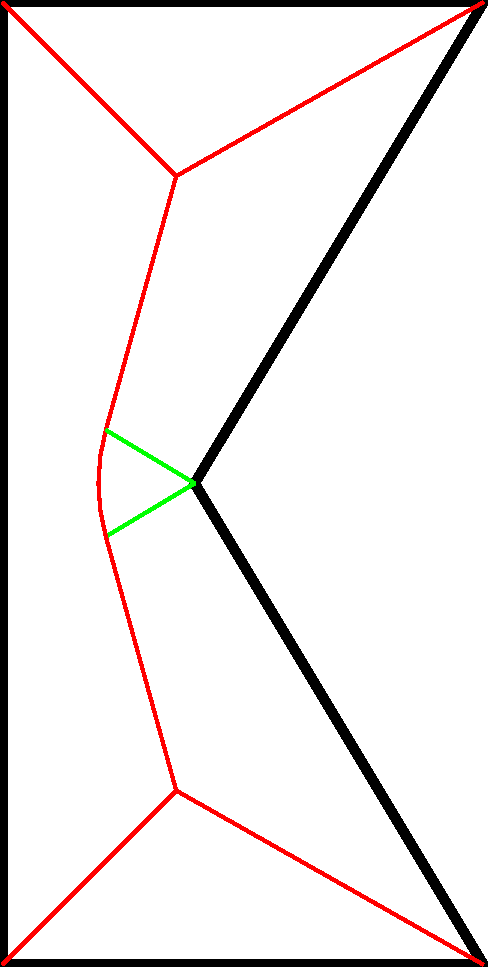
\includegraphics[height=\figwidthTwo]{sources-method-simple-skeleton-vd}
\caption{Voronoi Diagram}\label{shape_decomposition_vd}
\end{subfigure}
\begin{subfigure}[t]{\figwidth}\centering
\includegraphics[height=\figwidthTwo]{sources-method-simple-skeleton-st}
\caption{Skeletal Trapezoidation}\label{shape_decomposition_st}
\end{subfigure}
\begin{subfigure}[t]{\figwidth}\centering
\includegraphics[height=\figwidthTwo]{sources-method-half-edge-datastructure.pdf}
\caption{Data structure}\label{shape_decomposition_datastructure}
\end{subfigure}
\caption{
Skeletonization of an outline shape (black).
Relation between the medial axis (red), the limited Voronoi Diagram (red and green) and the Skeletal Trapezoidation (red, green and gray): MAT $\subset$ Limited VD $\subset$ ST.
\subref{shape_decomposition_datastructure} The skeleton is represented using a half-edge data-structure.
}
\label{skeletonization_comparison}
\end{figure}



%\subsubsection{Skeletal trapezoidation}
\paragraph{Skeletal trapezoidation}
Starting from the medial axis we decompose the input polygon into a set of quads and triangles, so that we can perform the slicing stage on simple shapes.
We employ a shape decomposition similar to the one proposed by \citeauthor{Ding2016a}~\cite{Ding2016a}. 
The basic idea is to add edges connecting each node $v$ on the medial axis to each of its support points $\text{sup}(v)$. 
The resulting skeleton decomposes the outline shape into trapezoids and triangles.
Considering the fact that the concept of trapezoidation conventionally allows for the degenerate case where a trapezoid resolves into a triangle~\cite{chazelle1984,fournier1984}, we call this shape decomposition the \emph{Skeletal Trapezoidation} (ST).


The edges generated by the MAT are classified into three types:
\begin{enumerate*}
\item line-line edge -- straight edge generated from two line segments in the outline polygons,
\item vertex-line edge -- parabolic edge resulting from an outline vertex and a line segment in the outline, and 
\item vertex-vertex edge -- straight edge resulting from two outline vertices.
\end{enumerate*}
The vertex-line and vertex-vertex edges are discretized into pieces with a length up to \revise{$d^\text{discretization}$}{\SI{0.2}{\milli\meter}, which gives an approximation error of only $\pm$\SI{0.01}{\milli\meter}}.
This allows to approximate the feature radius between two discretized nodes $v_0$ and $v_1$ by linear interpolation. 
Again we connect the newly inserted nodes to their support, which results in vertex-line regions and vertex-vertex regions such as depicted in \cref{legend}.



\begin{figure}\centering
\includegraphics[width=.75\columnwidth]{sources-method-legend2.pdf}
\caption{Illustrative explanation of terms and color coding that are consistently used in this paper.}
\label{legend}
\end{figure}




% The ST contains all edges from the medial axis which are generated from two line segments in the outline polygons.
% The interaction between an outline vertex and a line segment results in a parabolic edge, which is discretized into pieces with a length up to $d^\text{discretization}$ (see the middle of \cref{shape_decomposition_st}).
% Additionally medial axis edges which are generated from two outline vertices are also discretized, so that the feature radius $R$ in between two discretized nodes $v_0$ and $v_1$ can be approximated by linear interpolation between $R(v_0)$ and $R(v_1)$.
% Again we connect the nodes which are introduced by the discretization to their support, which results in vertex-line regions and vertex-vertex regions such as depicted in \cref{legend}.



%\subsubsection{Union of cones}
\paragraph{Approximation of union of cones}
The skeletal trapezoidation (ST) provides a means to visualize the union of cones (UoC) approximated by a 3D surface mesh composed of quadrilateral and triangular patches.
%In order to visualize the ST as a 3D surface, we add a third dimension.
We assign each node in ST a (real number) height value measured in terms of beads, referred to as the \emph{bead count} $b$.
We define the bead count as the number of beads to fit along the \emph{diameter} of the inscribed circle centered at node $v$, i.e. $2R(v)$, by
\begin{equation}
    \tilde{b}_v = 2 R(v) / w^*
\label{eq:initialBeadCount}
\end{equation}
where $w^*$ is the nozzle size. 
%While the feature radii are measured along the support edges, the diameter is not measurable as such because the support edges are generally not collinear;
We divide the diameter rather than the radius as this allows to deal with an odd number of beads while using integer logic.
%The result is a mesh representing the union of cones (UoC) consisting entirely of quads and triangles.
Note that although the overview of the method was described geometrically in terms of the UoC, the actual toolpath generation relies on the two-dimensional ST;
the use of the bead count as a height value is only a visualization aid.







\paragraph{Implementation}
The medial axis of a polygonal shape is a subset of the Voronoi Diagram generated from the line segments and vertices of the shape~\cite{lee1982medial}. 
The edges of the Voronoi diagram that fall outside of the outline shape are irrelevant for our purpose and \revise{}{are }thus discarded.
Note that besides the full medial axis, the Voronoi diagram also contains edges connecting to concave vertices in the outline shape (see \cref{shape_decomposition_vd}). 
These extra edges are a subset of the edges connecting a node to its support, so we keep them in.
From the Voronoi diagram we add nodes to discretize parabolic edges and edges formed by two concave outline vertices, and then connect all nodes to their supports, forming a skeletal trapezoidation. 
We then assign each node the bead count values using \cref{eq:initialBeadCount}.
We compute the Voronoi diagram using the Boost \verb!C++! libraries~\cite{schaling2011boost}, which implements the algorithm proposed by \citeauthor{fortune1986sascg}~\cite{fortune1986sascg}.
A half-edge data-structure is used to represent the Voronoi diagram (\cref{shape_decomposition_datastructure}).

%









\subsection{Center classification}\label{sec_center_classification}
%The simple technique of performing uniform width offset produces large overfill and underfill areas on central regions of the ST.
%These central regions present themselves as upper ridges in the mountains of the UoC surface.
%In order to prevent the over- and underfill we will change the bead counts in the central regions.
%This sections covers what parts of the UoC will be marked as being central.
In order to prevent over- and underfill \revise{to occur}{from occurring} in central\revise{}{ regions}, we mark parts of the ST as being central.
\revise{The remainder is called peripheral.}{}
Our framework will decide on a beading at all the marked nodes in `the center' and apply the beading outward to the unmarked nodes (\cref{sec_peripheral_height_adjustment}).

We mark a node in the ST as central if its feature radius is larger than that of all its neighboring nodes, i.e. a local maxima.
%That is: we mark the local maxima, i.e. the mountain tops of the UoC as being central.
We also mark an edge as being central if it is significant according to a significance measure.

%\subsubsection{Significance measure}\label{sec:significance_measure}
\paragraph{Significance measure}
We make use of the \emph{bisector angle} as an indicator of significance which is commonly used in shape analysis.
%Centrality can be formalized by looking at a commonly used significance measure knows as the \emph{bisector angle}.
The bisector angle $\alpha$ is the interior angle $\angle{p_0lp_1} \leq \SI{180}{\degree}$, between any location $l$ on an edge of the ST and its two supporting points $ \{ p_0, p_1 \} = \text{sup}(l)$~\cite{attali1996modeling}. 
An edge is significant if the bisector angle on any location on the edge exceeds a prescribed $\alpha_\text{max}$. 
As illustrated in \revise{See }{}\cref{naive_overfill_underfill}, for a polygon with a pointy wedge area of an angle $\beta$, we have $\alpha = 180\degree - \beta$.
This corresponds to overfill areas and underfill areas the size of \revise{$\nicefrac12 (w^*)^2 \left( \nicefrac14 \tan ( \alpha / 2) - \alpha / 2 \right)$}{$\nicefrac14 (w^*)^2 \left( \tan ( \alpha / 2) - \alpha / 2 \right)$} when filled using the simple technique of uniform bead width $w^*$.
\revise{}{A too large $\alpha_\text{max}$ may leave a lot of under-/overfill, while a too small value may introduce toolpaths to fill in negligibly small underfills.
We therefore set $\alpha_\text{max} = \SI{135}{\degree}$.}
Although significance measures are commonly used as a heuristic for finding the parts of a skeleton which are in some sense relevant~\cite{attali1996modeling,Sud2007},
we use the bisector angle as an \emph{exact} indicator of the amount of overfill and underfill in the uniform toolpaths of constant width.
%Contrary to related literature we will \emph{keep} the non-significant regions of the skeleton.
%We mark all significant edges as such and contrary to related literature we keep the unmarked edges of the ST.


\begin{figure}
\centering
\setlength{\figheight}{.3\columnwidth}
\begin{subfigure}{0.45\columnwidth} \centering
\includegraphics[height=\figheight,frame]{sources-method-naive-overfill-underfill.pdf}
\caption{Over- and underfill}\label{naive_overfill_underfill}
\end{subfigure}
\begin{subfigure}{0.45\columnwidth} \centering
\includegraphics[height=.8\figheight]{sources-method-significance-properties.pdf}
\caption{Significance measure}\label{distance_based_angles}
\end{subfigure}
\caption{
Properties of the significance measure along a skeletal edge (red) generated from two polygon lines (black) using the properties of inscribed circles (gray) and their radii (dashed).
\subref{naive_overfill_underfill}
The size of overfill (orange) and underfill areas (azure) for the uniform toolpathing technique can be calculated from the bisector angle.
% $a = 180\degree - \beta$ is the angle between a location $v$ and its support $p_0$ and $p_1$.
\subref{distance_based_angles}
The significance measure can be simplified using $\alpha = 2 \gamma = 2 \cos^{-1} \Delta R / |v_1 - v_0|$.
}
\end{figure}

% The significance evaluation is performed efficiently by checking the ratio between feature radius $R$ and the Euclidean distance:
% if $ | R(v_1) - R(v_0) | / |v_1 - v_0| >  \cos(\alpha_\text{max} / 2)$ then $\alpha > \alpha_\text{max}$. See \cref{distance_based_angles}. This ratio has a clear geometrical interpretation as the slope of the ridge in the UoC surface.

To avoid evaluating the bisector angle at any location on all edges, we devise an efficient measure which operates only on the two nodes of an edge.
Because all locations along a line-line edge have the same bisector angle we can evaluate whether the edge is significant by checking whether 
\begin{align}\label{simple_significance_measure}
| R(v_1) - R(v_0) | / |v_1 - v_0| >  \cos(\alpha_\text{max} / 2)
\end{align}
(see \cref{distance_based_angles}).
This ratio has a clear geometrical interpretation as the slope of the ridge in the UoC surface.
For vertex-line edges and vertex-vertex edges only a portion of the edge is significant.
We therefore introduce nodes at the boundaries of the significant portion during the discretization of such edges (see Appendix~\ref{edge_discretization}).
The significance of all edges can then accurately be evaluated using \cref{simple_significance_measure}.






%\subsubsection{Marking filtering}
\paragraph{Marking filtering}
After initializing the marking at all edges and nodes, we filter out high frequency changes in the marking in order to ensure that the generated toolpath is smooth. 
The filtering is performed by additionally marking some unmarked elements, rather than the opposite since unmarking central regions reintroduce\revise{}{s} large over- and underfill areas.
From each marked node $v_0$ with an upward unmarked edge attached we walk along the upward edges;
if the total length traversed until we reach another marked node $v_1$ is shorter than some filter distance $d_\text{max}^\text{unmarked}$, we mark all edges encountered as being central.
\revise{}{We use $d_\text{max}^\text{unmarked} = w^*$ in order to filter out high frequency oscillations in the order of magnitude of the nozzle size, while keeping close to the significance measure.}














\subsection{Central height adjustment}\label{sec_central_height_adjustment}
Now that we have identified and marked the central regions\revise{}{,} we quantize their heights.
We first quantize the initial bead count $\tilde{b}$ into an integer bead count $\bar{b}$ at the marked nodes using a quantization operator $q$,
then find the locations along the edges where $q$ makes a jump from one bead count $n$ to another $n+1$
and then introduce ramps to smoothly transition from $n$ to $n+1$ using fractional bead counts $\hat{b}$ along the smooth transition.
%\subsubsection{Initial bead count}\label{sec_initial_bead_count}



\begin{figure*}
\centering
\setlength{\figwidth}{0.13\textwidth}
\begin{subfigure}{\figwidth}
\includegraphics[width=\columnwidth]{sources-method-beading-transitioning-filtering--bead-count.pdf}
\caption{Quantized bead counts}\label{beading_transitioning_filtering__bead_count}
\end{subfigure}
\begin{subfigure}{\figwidth}
\includegraphics[width=\columnwidth]{sources-method-beading-transitioning-filtering--transition-mids.pdf}
\caption{Transition anchors}\label{beading_transitioning_filtering__transition_mids}
\end{subfigure}
\begin{subfigure}{\figwidth}
\includegraphics[width=\columnwidth]{sources-method-beading-transitioning-filtering--filtered.pdf}
\caption{Filtered anchors}\label{beading_transitioning_filtering__filtered}
\end{subfigure}
\begin{subfigure}{\figwidth}
\includegraphics[width=\columnwidth]{sources-method-beading-transitioning-filtering--transition-ends.pdf}
\caption{Transition ramp ends}\label{beading_transitioning_filtering__transition_ends}
\end{subfigure}
\begin{subfigure}{\figwidth}
\includegraphics[width=\columnwidth]{sources-method-beading-transitioning-filtering--transitions-applied.pdf}
\caption{Radial support edges}\label{beading_transitioning_filtering__transitions_applied}
\end{subfigure}
\begin{subfigure}{.27\textwidth}
\hspace*{-.5cm}\includegraphics[width=1.2\columnwidth]{sources-method-beading-transitioning-filtering--result-uoc.pdf}
\caption{Result UoC}\label{beading_transitioning_filtering__result_uoc}
\end{subfigure}
\caption{
Applying bead counts and transitioning on a shape showing the difference between a simple ST (top) and a mirrored version with small perturbations in the outline (bottom).
Outline in black, central edges marked in blue, radial edges in grey.
\subref{beading_transitioning_filtering__bead_count} First we initialize the bead counts (black) in the marked edges (blue).
\subref{beading_transitioning_filtering__transition_mids} We then extract the anchor locations (purple) where the bead count transitions.
\subref{beading_transitioning_filtering__filtered} We then filter out regions which exhibit frequent transition.
\subref{beading_transitioning_filtering__transition_ends} We then calculate the end locations (magenta, pink) of the transitions and modify the bead count at nodes in between to fractional values.
\subref{beading_transitioning_filtering__transitions_applied} Finally we introduce nodes at the ends and introduce radial edges (purple) as per the trapezoidation constraint.
The symmetry in the result shows that transitioning is robust against small perturbations in the outline shape.
}
\label{beading_transitioning_filtering}
\end{figure*}


%\subsubsection{Quantization}

\paragraph{Quantization}
We define a quantization operator $q$ to map a feature diameter ($d=2R(v)$) to a bead count: $q: \mathbb{R} \to \mathbb{N}$.
Because our quantization scheme should round to the nearest integer multiple of the nozzle size, we have
$q(d) = \left\lfloor d / w^* + \nicefrac12 \right\rfloor$.
Alternative quantization schemes are discussed in \cref{sec_generalization}.
By applying $q$ to the heights of central nodes we quantize the bead count:
\begin{equation}\label{eq_quantized_bead_count}
\bar{b}_v = q(2R(v)) = \left\lfloor \tilde{b}_v + \nicefrac12 \right\rfloor
\end{equation}

\iffalse
Along with this quantization, an amendment to the marking filtering is performed, in order to alleviate a problem that will be handled in \cref{section_beading_conflicts}.
Specifically, unmarked regions are marked as central if they lie between two nodes with the same integer bead count.
\fi
%We then filter out short unmarked regions where the bead count remains constant in order to limit the extent of a problem handled in \cref{section_beading_conflicts}.
% From each marked node $v_0$ with an upward unmarked edge attached we walk along the upward edges until we hit another marked node $v_1$.
% If the upper node has the same bead count $b^*_{v_1} = b^*_{v_0}$ we mark all edges and nodes $v$ in between, and set the bead count $b^*_v \leftarrow b^*_{v_0}$.

\paragraph{Transition anchors}
For a marked edge which connects nodes $v_0$ and $v_1$ with $\bar{b}_{v_0} \le n < \bar{b}_{v_1}$, we determine the \emph{transition anchor locations} at which the bead count transitions from $n$ to $n+1$.
To this end, we introduce the function 
\begin{equation}
    q^{-1}(n) := \argmax_d q(d) = n,
\end{equation}
which gives the feature diameter $d$ at which the bead count $q$ transitions from $n$ to $n+1$.
The location of the anchor $v_x$ is then computed by inversely interpolating $R(v_x) = q^{-1}(n)$, i.e. 
\begin{equation}
    v_x = v_0 + (v_1 - v_0) \frac{ q^{-1}(n) - R(v_0) }{ R(v_1) - R(v_0) }.
\end{equation}
%for each $n$ such that $b^*_{v_0}\le n<b^*_{v_1}$.
An illustration of the anchors is shown in \cref{beading_transitioning_filtering__transition_mids}.

We perform a filtering step to prevent frequently changing the bead count back and forth within a short distance.
For two consecutive anchors which transition to opposite directions, if the distance between them is smaller than some limit $d_\text{max}^\text{transition}$, the bead counts at all nodes in-between are set to the surrounding bead counts, and consequently these anchors are removed (See \cref{beading_transitioning_filtering__filtered}).
\revise{}{A value of $d_\text{max}^\text{transition} = \SI{1}{\milli\meter}$ seems to produce satisfactory results.}
\revise{}{This means that for some small regions we generate toolpaths with bead widths outside the typical range.}

% For each edge which contains a transition anchor we walk along the marked edges until we encounter another anchor.
% If the other anchor is a transition in the opposite direction and the traversed distance is within some limit $d_\text{max}^\text{transition}$ we remove the transitions and set the bead counts at all nodes in the filtered region to the surrounding bead counts.
% See \cref{beading_transitioning_filtering__filtered}.






% \subsubsection{Smooth transition}
\paragraph{Smooth transitions}

A sharp transition from $n$ to $n+1$ beads at an anchor location creates sharp turns in the toolpath (see \cref{transitions} top).
We introduce a transition length $t(n)$ to ensure a smooth transition (see \cref{transitions}). 
The length of the transition is set to $t(n) = w^*$ and it is centered at the anchor, i.e. the distance from the lower end $v_0$ to the anchor position $v_x$ is set to
\revise{$t_0(n) = \Delta(v_0v_x) = \nicefrac12 w^*$,}
{$t_0(n) \equiv \Delta(v_0v_x) =  t(n) \left( q^{-1}(n) / w^*  - n \right)$,}
where $\Delta$ is the total distance along the edges between two nodes.
\revise{}{The transition length $t(n)$ ensures that the center beads don't overlap with the innermost transitioning beads, while keeping the amount of underfill low and the toolpath smooth.
The transition anchor position $t_0(n)$ ensures that the transitions never overlap with each other or with locations where all beads have the preferred width $w^*$.}


We discard any transition anchor which is too close to the end of a chain of marked edges for the smoothed transition to fully fit within the marked region.
In order to make the transition ramps robust against small perturbations in the outline shape which cause extra (support) edges in the skeleton,
we modify the nodes $v_x$ which are between the two ends $v_0$ and $v_1$ of the transition by (re-)assigning them a fractional bead count $\hat{b}$ which is linearly interpolated between the two ends of the transition (see \cref{beading_transitioning_filtering__transitions_applied}):
\begin{equation}
\hat{b}_{v_x} = n + {\Delta(v_0v_x)} / {\Delta(v_0v_1)}
\end{equation}
Note that although the ST is not stable against noise in the boundary shape, the distance field itself is, so by designing our algorithms such that they are stable against changes in the topology of the skeleton our method is stable against small perturbations in the outline.
%This modification makes the transition ramps robust against small perturbations in the outline shape (to be explained in \cref{section_beading_interpolation});
%compare the top and bottom of \cref{beading_transitioning_filtering}. 
Finally we update the ST by adding support edges at the transition ends. 
As shown in \cref{beading_transitioning_filtering__result_uoc}, the marked regions in the UoC mesh have become horizontal at integer multiples of $\nicefrac12 w^*$ for long stretches with ramps in between.




\begin{figure}
\centering
\setlength{\figwidth}{\columnwidth}
\begin{subfigure}{0.9\figwidth}\centering
\includegraphics[width=\columnwidth]{sources-method-wedge-no-transitioning.png}
\caption{Without transitioning}
\end{subfigure}
\begin{subfigure}{0.9\figwidth}\centering
\includegraphics[width=\columnwidth]{sources-method-wedge-transitioning.png}
\caption{Transitioning}
\end{subfigure}
\caption{
Sharp turns around regions where the bead count changes are prevented by transition regions (highlighted in cyan).
}
\label{transitions}
\end{figure}














\subsection{Beading}\label{sec_peripheral_height_adjustment}
Now that we have determined the bead counts in the \revise{}{marked }central regions we will describe how the \revise{peripheral}{unmarked} regions are handled.
Determining bead count values for the unmarked nodes and interpolating linearly along the unmarked edges would mean that toolpath sites would be distributed evenly along each unmarked bone;
while that would suffice for the evenly distributed beading scheme, it wouldn't allow for more sophisticated, non-linear schemes.
Instead we determine the radial distance to the boundary at which each bead should occur from the boundary to the center.
Each central node is associated with a sequence of radial distances $L$ which control the locations of the beads, starting from the outer bead and ending in the center.
Together with a sequence of bead widths $W$\revise{}{,} these form what we call a \emph{beading} $B$.
For our distributed beading scheme we compute the beading for a central node $v$ with $n = \lfloor \hat{b}_v \rfloor$ beads and a diameter $r = R(v)$  as:
\begin{align*}
    B(n,r) &= \left( W(n,r), L(n,r) \right)   &=   \left( \left\{  w_0  \dots w_{\lceil n/2 \rceil-1} \right\}, \left\{ l_0 \dots l_{\lceil n/2 \rceil-1} \right\} \right) \\
    w_i &= r / n  & \text{for all $i \in \mathbb{N} : i < n / 2 $}\\
    l_i &= r / n (i + \nicefrac12) & \text{for all $i \in \mathbb{N} : i < n / 2 $}
\end{align*}
where
$w_i$ and $l_i$ are the width and location of the $i$th bead,
respectively, counting from the outline inward.
Example beadings for an odd and even bead count with arbitrary widths are visualized in \cref{example_beading}.





\paragraph{Beading interpolation}
The beading is defined in terms of an integer number of beads, while we have assigned a fractional bead count to nodes within a transition region.
In order to generate a beading for a node $v$ with $n < b^*_v < n+1 $ we linearly interpolate the bead widths and locations between a beading $B^1$ based on $n$ and a beading $B^2$ based on $n+1$ (see \cref{beading_interpolation}).
Such interpolation is also used to deal with beading conflicts (see \cref{beading_conflict_problem}).
There we also apply beading interpolation from a marked node $v_m$ upward along unmarked bones,
and interpolate between $v_m$ and the beading at the top of the slope over some distance $t_\text{beading}$ from the lower marked node\revise{.}{, which we set to $t_\text{beading} = w^* $, so that the transition is not too swift.}

\paragraph{Beading propagation}
The beading information is then broadcast throughout the ST from central regions outward,
so that each unmarked node $v$ knows the beading of the marked node on top of the ramp on which $v$ is placed.
We first broadcast the beading information upward from all marked nodes,
so that we can then deal with beading conflicts in a downward phase.
\revise{This the}{The} downward phase makes sure that all nodes have a beading associated with it, so that the slicing algorithm can efficiently slice the edges leading up to a marked or unmarked node.	



\begin{figure}
\centering
\setlength{\figheight}{.29\columnwidth}
\begin{subfigure}{0.4\columnwidth}\centering
\includegraphics[height=\figheight]{sources-method-trapezoid-beading-interpolation-beading.pdf}
\caption{Example beadings}\label{example_beading}
\end{subfigure}
\begin{subfigure}{0.4\columnwidth}\centering
\includegraphics[height=\figheight]{sources-method-trapezoid-beading-interpolation.pdf}
\caption{Interpolation}
\end{subfigure}
\caption{
Interpolation between two beadings $B^1$ and $B^2$ with odd and even bead count resulting in a beading $B^x$ at $n+\nicefrac23$.
Bead indices are counted inward from the outline (thick black).
Interpolation of locations in dots, interpolation of widths in dashes.
}
\label{beading_interpolation}
\end{figure}

\begin{figure}\centering
\setlength{\figheight}{.2\columnwidth}
\begin{subfigure}{.45\columnwidth}\centering
\includegraphics[width=.95\columnwidth,frame]{sources-method-beading-conflict-3D.png}
\includegraphics[height=\figheight]{sources-method-beading-conflict.pdf}
\caption{Beading conflict}\label{beading_conflict}
\end{subfigure}
\begin{subfigure}{.45\columnwidth}\centering
\includegraphics[width=.95\columnwidth,frame]{sources-method-beading-conflict-solved-3D.png}
\includegraphics[height=\figheight]{sources-method-beading-conflict-solved.pdf}
\caption{Conflict resolution}\label{beading_conflict_solved}
\end{subfigure}
\caption{
\subref{beading_conflict} The beading propagated from above conflicts with the beading below.
\subref{beading_conflict_solved} The beading conflict is resolved by gradually interpolating between the two beadings.
The ramp to the upper ridge doesn't line up with the lower ridge, which means that
the toolpaths (dashed) resulting from the beading propagated from above doesn't align with the beading from the thin outline feature (highlighted in red).
}
\label{beading_conflict_problem}
\end{figure}








\subsection{Toolpath extraction}\label{sec_toolpath_extraction}
Now that each node has been assigned a beading we proceed to generate the toolpath sites along the edges of the ST.
A site $S$ consists of a location $v$ a width $w$ and an index $i$, which are computed for an edge $v_0v_1$ from the beading $B$ of the upper node $v_1$:
\begin{align*}
S &= \{ v, w, i \} \\ 
v &= v_1 + (v_0 - v_1) \frac{R(v_1) - l_i^B}{R(v_1) - R(v_0)} \\ 
w &= w_i^B
% \\ i^S &= i
\end{align*}
for any $i$ for which $R(v_0) < l_i^B \leq R(v_1)$.
See \cref{site_placement}.
We store all sites of an edge in a mapping from edge to a list of sites.


\begin{figure}
\centering
\setlength{\figheight}{.29\columnwidth}
\begin{subfigure}{0.14\columnwidth}\centering
\includegraphics[height=\figheight]{sources-method-trapezoid-beading-beading.pdf}
\caption{Beadings}\label{trapezoid_beading_beading}
\end{subfigure}
\begin{subfigure}{0.5\columnwidth}\centering
\includegraphics[height=\figheight]{sources-method-trapezoid-beading-propagated.pdf}
\caption{Single beading propagated to all nodes}\label{trapezoid_beading_propagated}
\end{subfigure}
\begin{subfigure}{0.34\columnwidth}\centering
\includegraphics[height=\figheight]{sources-method-trapezoid-beading-separate.pdf}
\caption{Separate beadings at either top node}\label{trapezoid_beading_separate}
\end{subfigure}
\caption{
Applying beadings to generate sites along trapezoids.
\subref{trapezoid_beading_beading} shows the locations $l_i$ and widths $w_i$ of two arbitrary different beadings.
\subref{trapezoid_beading_propagated} shows the application of $B^1$ to the various types of trapezoid.
\subref{trapezoid_beading_separate} shows how a trapezoid with a marked edge will have two different beadings assigned, which will generate their respective sites along the support edges.
No sites will be generated along marked edges.
Wide black lines are outline segments, marked nodes and edges in blue, the sites in yellow and green wavefronts of equidistant radial distance at $R = l_i$.
}
\label{site_placement}
\end{figure}


We then generate extrusion segments for each trapezoid by connecting together the sites of the same index.
See \cref{segment_generation}.
If the amount of sites on both sides of the trapezoid is not the same then this trapezoid is in a transition and we leave one inner site unconnected.

Because the bead count is defined in terms of the feature diameter rather than the radius, only some of the bead count values $\hat{b}$ in a central region coincide with a slicing height.
When the bead count $\hat{b}$ is even, the ridge is sliced as normal;
the intersection between a slicing plane and the mesh surface results in a polyline on both sides of the ridge, which are connected together into a polygonal toolpath.
When the bead count $\hat{b}$ is odd, the ridge will coincide exactly with a slicing height, which results in a single polyline toolpath being generated along the middle of the feature.
In that case we should prevent the algorithm from generating the center extrusion segment twice from the trapezoids on either side of that segment.
We therefore use some arbitrary condition to decide which one of the two to include based on the ordering of the coordinates of $v_0$ and $v_1$: $x_0 < x_1 \lor (x_0 = x_1 \land y_0 < y_1)$.

All trapezoids in the ST are assigned to separate domains, corresponding to which boundary polygon they are connected to (see \cref{shape_decomposition_domains})~\cite{Ding2016a}.
By traversing the trapezoids \revise{in }{}per domain in order we can efficiently connect all segments into polylines.
See \cref{segment_generation}.
In a final step we connect the ends of polylines together, so that the final toolpaths contain both polygons and polylines.

\begin{figure}
\centering
\setlength{\figheight}{.3\columnwidth}
\begin{subfigure}{.5\columnwidth}\centering
\includegraphics[width=\figheight,rotate=90]{sources-method-domains.pdf}
\caption{Polygon domains}\label{shape_decomposition_domains}
\end{subfigure}
\begin{subfigure}{.45\columnwidth}\centering
\includegraphics[height=\figheight]{sources-method-segment-generation.pdf}
\caption{Extrusion segment chaining}\label{segment_generation_chaining}
\end{subfigure}
\caption{
Generating toolpaths on a part of the test outline shape by chaining together extrusion segments along each polygon domain.
Each edge is assigned toolpath sites (yellow) which are connected together as shown in the singled out trapezoid.
By following the trapezoids along the domain (cyan) of a single outline polygon,
the extrusion segments can efficiently be connected into existing polyline toolpaths (light and dark gray).
}
\label{segment_generation}
\end{figure}


Around the transition locations and around nodes with odd bead count and more than two marked edges attached there will be intersections in the toolpaths.
Such intersections cause overfill because the nozzle passes the location multiple times.
We deal with this special case by forcing a new polyline when traversing the trapezoids, and in the final polyline connection step we greedily connect the first two polylines ending in the same location and retreat all other polylines ending in that same location in order to prevent the overfill.
In order to retreat a polyline which ends in a site $S$\revise{}{,} we remove part of the polyline paths up to the intersection by a distance of $w^S d_\text{max}^\text{intersection}$\revise{, where $d_\text{max}^\text{intersection}$ is some ration between $0$ and $1$.}{.
We set $d_\text{max}^\text{intersection} = \SI{75}{\percent}$ in order to slightly favor overfilling over underfilling.}
This ratio effectively deals with the balance between overfill and underfill generated at that location after the retreat has been applied.
See \cref{polyline_reduction}.


\begin{figure}
\centering
\setlength{\figwidth}{.35\columnwidth}
\begin{subfigure}{0.45\columnwidth}\centering
\includegraphics[width=\figwidth,frame]{sources-method-polyline-reduction-before}
\caption{No reduction}
\end{subfigure}
\begin{subfigure}{0.45\columnwidth}\centering
\includegraphics[width=\figwidth,frame]{sources-method-polyline-reduction-after}
\caption{Reduction}
\end{subfigure}
\caption{
Reducing polyline toolpaths away from intersections in order to prevent overfill.
Toolpath locations in black, underfill in azure and overfill in orange.
}
\label{polyline_reduction}
\end{figure}





























































\section{Generalization}\label{sec_generalization}
In this section we will generalize the described method into a parametric system, i.e. an algorithmic framework.
The method we have described above is one for distributing the beads evenly over the total diameter of an outline shape feature.
Depending on the application, the hardware and the materials used we might need different strategies for determining the bead widths.
In this section we will generalize the method so that we can apply any distribution of bead widths over a feature radius.
There are several strategies one can take for determining the distribution of bead widths.
We will formalize several strategies and describe the set of parameters these strategies require.


\begin{definition}\label{beading_strategy_definition}
We define a beading strategy as the following set:
$$
\left\{ \alpha_\text{max}, f(d), t(n), t_0(n), W(n, d), L(n, d) \right\}
$$
where
$\alpha_{\text{max}}$ (the limit bisector angle),
$f(d)$ (flattening operator),
$t(n)$ (transition length)
and
$t_0(n)$ (transition anchor position) have already been defined above.
We introduce here
$W(n, d)$, which gives the sequence of bead widths $\left\{ w_i \right\}$ for each bead with index $i$
and
$L(n, d)$, which gives the sequence of radial locations $\left\{ l_i \right\}$ which map to each bead index $i$.
\end{definition}


The following restrictions hold:
\begin{enumerate}
\item $\alpha_\text{max}$ is viable: $t_1(n) + t_0(n+1) < \frac{ f^{-1}(n + 1) - f^{-1}(n) }{ \cos \nicefrac12 \alpha_\text{max}}$ for each $n \in \mathbb{N}$ (see \cref{transition_placement})
\item $W$ is symmetric: $W(n, d)_i = W(n, d)_{n-i-1}$
\item $L$ is symmetric in $d$: $L(n, d)_i = d - L(n, d)_{n-i-1}$
\item $W_n$ is monotonic and continuous at each bead index $n$ for constant bead count $c$: $0 \leq \frac{\partial W(c, d)_n}{\partial d} < \infty$
\end{enumerate}



\begin{figure}
\centering
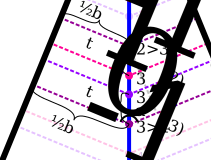
\includegraphics[width=.4\columnwidth]{sources/method/transition_length_limit.pdf}
\caption{
Placement of transition ends (magenta and pink) with respect to the anchor positions of the transitions (purple) on a ST edge (blue) with bisector angle $\alpha \approx \SI{135}{\degree}$.
The distance between the anchor position and the upper end ($t_1$) and the distance between the anchor position and the lower end of the transition ($t_0$) should add up to less than the total distance between the anchor positions, which is limited by $\alpha_\text{max}$.
}
\label{transition_placement}
\end{figure}


Because the peripheral height adjustment was described in terms of a mapping from radial distances to junctions rather than adjusting the heights of peripheral nodes,
we can introduce non-linear mappings without refining the surface mesh.
In the simplified geometrical conceptualization of our technique we can introduce different distributions of bead widths from the center outward, by making the contours of the cones curved.
If the UoC mesh is generated with cones which are curving inward toward the top, higher slicing planes would intersect more sparsely than lower ones, which means that the inter-bead distance and thus their width becomes larger when going inward.
In order for the simplified geometrical approach to capture such curved shapes it would have to perform mesh refinement.
However, our approach bypasses the peripheral height adjustment and directly generates the radial distances at the slicing heights, which means our technique generalized effortlessly.




\subsection{Beading strategies}
We introduce several beading strategies which determine the bead count and their widths in various ways.
We can emulate a variety of toolpath generation methods from related literature by defining new beading strategies.
We also introduce new beading strategies which produce toolpaths with less extremal widths compared to techniques from existing literature.

A beading strategy is defined as a set of some particular variables and functions (\cref{beading_strategy_definition}).
Our beading strategies are based on a preferred width $w_\text{pref} = \SI{0.4}{\milli\meter}$, which is equal to the diameter of the printing nozzle.
Most of the beading strategies we introduce share a common ground:
\begin{align*}
d_\text{max}^\text{transition} &= \SI{1}{\milli\meter} \\
d^\text{discretization} &= \SI{0.2}{\milli\meter} \\
t_\text{beading} &= w_\text{pref} \\
d_\text{max}^\text{intersection} &= \SI{75}{\percent} \\
%
%We use a transition anchor position of
%$$t_-(n) =  t(n) \frac{ f^{-1}(n) - p(n) }{p(n+1) - p(n) }$$
%$$t_-(n) =  t(n) \frac{ f^{-1}(n) - 0.4n }{0.4(n+1) - 0.4n }$$
%$$t_-(n) =  t(n) \frac{ f^{-1}(n) - 0.4n }{0.4}$$
t_0(n) &=  t(n) \left( f^{-1}(n) / w_\text{pref}  - n \right) \\
t(n) &= w_\text{pref} \\
\alpha_\text{max} &= \SI{135}{\degree} \\
L(n,d)_i &= 
\begin{cases}
-\frac12 W(n,d)_i + \sum_{j=0}^i W(n,d)_j & \text{ if } i < \frac12 (n -1) \\
d/2 & \text{ if } i =  \frac12 (n -1) \\
d - W(n,d)_{n-1-i} & \text{ otherwise }\\
\end{cases}
\end{align*}

The transition anchor position $t_0$ ensures that the transitions never overlap with the locations $v$ where $2 R(v) = n w_\text{pref}$ for $n \in \mathbb{N}$.
The transition length $t$ ensures that the center beads don't overlap with the innermost transitioning beads, while keeping the amount of underfill low and keeping the toolpath smooth.
The limit bisector angle $\alpha_\text{max}$ ensures that we don't employ transitioning in shallow wedge regions, which would result in a lot of short odd single bead polylines, which would break up the semi-continuous nature of polygonal extrusion paths.
The toolpath locations $L$ ensure that beads are extruded from the center of where they end up, that the beads don't overlap and that the symmetry restrictions are met.


\paragraph{Naive Beading Strategy}
We can define a beading strategy which emulates the naive method by disabling the marking of edges, so that we never employ transitioning.
\begin{align*}
\alpha_\text{max} &= \SI{180}{\degree} \\
f^-(d) &= 2 \left\lfloor \frac{d}{ 2w_\text{pref}} + \frac12 \right\rfloor \\
W(n,d)_i &= w_\text{pref} \text{ for all } i 
%\\
%L(n,d)_i &= w_\text{pref} \left(i + \frac12 \right) \text{ for all } i < \frac12 n
\end{align*}



\paragraph{Outer bead}
We can emulate the method by \citeauthor{Moesen2011} by carefully choosing how the beading strategy functions deal with the outermost bead.
Also we turn off the reduction of toolpaths near 3-way intersections, so that the polygonal toolpaths emulate the remaining area to be filled by another path planning technique similar to their technique.

\begin{align*}
d_\text{max}^\text{intersection} &= \SI{0}{\percent} \\
t(n) &= 0 \\
f(d) &=
\begin{cases}
1 & \text{ if } d < w_\text{pref} \\
2 & \text{ otherwise } \\
\end{cases}
 \\
W(n,d)_i &= 
\begin{cases}
d & \text{ if } n = 1 \\
w_\text{pref} & \text{ otherwise } \\
\end{cases}
%\\
%L(n,d)_i &= 
%\begin{cases}
%d / 2 & \text{ if } n = 1 \\
%w_\text{pref} / 2 & \text{ otherwise } \\
%\end{cases}
\end{align*}


\paragraph{Constant bead count}
We can emulate the method by \citeauthor{Ding2016a}, by dividing the feature diameter over the widths of a constant number of beads.
Additionally in order to emulate their definition of branches we mark all ST edges and in a separate algorithm we unmark the outer edges connected to the outline shape.
Note that this deviation from the proposed framework violates the robustness against small perturbations in the outline polygon, since the topology of the graph of the ST is not stable against those.

\begin{align*}
\alpha_\text{max} &= \SI{0}{\degree} \\
f(d) &= C \\
W(n,d)_i &= d / n \text{ for all } i 
%\\
%L(n,d)_i &= d / n \left(i + \frac12 \right) \text{ for all } i < \frac12 n
\end{align*}



\paragraph{Centered}
We can emulate the method by \citeauthor{Jin2017JMS}, by transcribing how they deviate from the naive tool paths.
We therefore base the beading strategy on the bead count $f^-(d)$ defined by the naive beading strategy.
\citeauthor{Jin2017JMS} replace two beads from the naive toolpaths by a single one when the radius between the center and either of those beads falls short of $r_\text{min} = 0.8 w_\text{pref}$.
Conversely, they place an extra bead when the radius between the center and either of the innermost beads exceeds $r_\text{max} = 1.25 w_\text{pref}$.\cite{Jin2017JMS}
We emulate the rounded polygonal path rerouting they define by supplying a transition length which results in a discretized version of the rounded polygon segment.

\begin{align*}
t(n) &= \frac12 w_\text{pref} \\
f^-(d) &= 2 \left\lfloor \frac{d}{ 2w_\text{pref}} + \frac12 \right\rfloor \\
f(d) &= f^-(d) +
\begin{cases}
-1 & \text{ if } f^-(d) w_\text{pref} - d > w_\text{pref} - r_\text{max} \\
1  & \text{ if }  f^-(d) w_\text{pref} - d < w_\text{pref} - r_\text{min} \\
0 & \text{ otherwise}
\end{cases}
\\
W(n,d)_i &= 
\begin{cases}
d - (n-1) w_\text{pref} &\text{ if } i = \frac12 (n-1) \\
w_\text{pref} &\text{ otherwise }
\end{cases}
%\\
%L(n,d)_i &= 
%\begin{cases}
%d / 2 & \text{ if } i = \frac12 (n-1) \\
%w_\text{pref} \left(i + \frac12 \right) & \text{ otherwise }
%\end{cases}
\end{align*}





\paragraph{Evenly distributed}
By taking the advantages of the above two strategies we can define a beading strategy which constitutes a novel toolpathing technique.
We can evenly divide the local feature diameter over the widths of all beads, but choose a local bead count better matching the local feature size.
We determine the local bead count by dividing the diameter by the prefered bead width and rounding to the nearest integer.
This reduces the demands on the system and deviation from mechanical properties caused by beads with extreme deviations from the preferred width.



\begin{align*}
f(d) &= \left\lfloor \frac{d}{ w_\text{pref}} + \frac12 \right\rfloor \\
W(n,d)_i &= d / n \text{ for all } i 
%\\
%L(n,d)_i &= d / n (i + \frac12) \text{ for all } i < \frac12 n
\end{align*}




\paragraph{General distributed strategy}
The evenly distributed strategy can be conceptualized as calculating the total discrepancy $E$ between the actual feature diameter $d$ and the total preferred width $n w_\text{pref}$, dividing the total discrepancy by the number of beads and setting the width of each bead to 
$w_\text{pref} + E / n$.
However, depending on the application we might want a different distribution of widths.
We therefore supply a beading strategy which supports an arbitrary distribution of the discrepancy.
The distribution is determined by some weighing function $M(n.d)$, which defines the portion of the discrepancy to distribute to each bead.


\begin{align*}
f(d) &= \left\lfloor \frac{d}{ w_\text{pref}} + \frac12 \right\rfloor \\
E(n,d) &= d - n w_\text{pref} \\
W(n,d)_i &= w_\text{pref} + E(n,d) \frac{M(n,d)_i}{\sum_{j=0}^{n-1} M(n,d)_j} \text{ for all } i 
%\\
%L(n,d)_i &= d / n (i + \frac12) \text{ for all } i < \frac12 n
\end{align*}


\paragraph{Inward distributed}
For example, we can choose 
$$M(n,d)_i = \max(0, 1 - \frac{1}{N^2} (i - (n-1)/2)^2 )$$
to distribute the discrepancy over the innermost $2N$ beads, and distribute most of it to the inner beads.
See \cref{distributed_comparison}.
That way we limit the region of impact of the distributed strategy to a central region and have the nominal bead width $w_\text{pref}$ in regions farther away.
This limits the impact of transitioning regions so that transitions keep the toolpaths smooth farther away from the central regions. % and it forces most of the beads to have exactly the prefered width.
Moreover, the bead widths equal the nominal bead width for large regions meaning that mechanical properties derived for prints using the naive strategy will still hold approximately.



\begin{figure}
\centering
\setlength{\figwidth}{.4\columnwidth}
\setlength{\figheight}{.25\columnwidth}
\begin{subfigure}{\figwidth}\centering
\includegraphics[height=\figheight]{sources/validation/wedge_Distributed_pretty_evenly.png}
\caption{Evenly distributed}
\end{subfigure}
\begin{subfigure}{\figwidth}\centering
\includegraphics[height=\figheight]{sources/validation/wedge_Distributed_pretty_inward.png}
\caption{Inward distributed}
\end{subfigure}
\begin{subfigure}{.1\columnwidth}\centering
\includegraphics[height=\figheight]{sources/validation/wedge_Distributed_pretty_legend.png}
\end{subfigure}
\caption{
Closeup of toolpaths generated with the distributed beading strategies for a large wedge shape.
Colors represent bead widths.
}
\label{distributed_comparison}
\end{figure}





\paragraph{Widening}
Complementary to any of these strategies we can enforce a minimum feature size at no extra cost in our framework.
Regions where the model is narrower than the nozzle size can be printed with a bead width larger than the model thickness.
We can simply override
\begin{align*}
W'(n,d)_1 &=
\begin{cases}
\max \left( w_\text{nozzle}  ,  W(n,d)_1 \right) & \text{ if } n = 1 \\
W(n,d)_1 & \text{ otherwise}
\end{cases}
\end{align*}






















\section{Validation}


\subsection{Strategies}
We can emulate a variety of toolpath generation strategies by applying various beading strategies to our framework.

\paragraph{Naive Strategy}


\paragraph{Constant bead count}
Emulates \cite{Ding2016a}


\paragraph{Deviation at middle}
Emulates \cite{Jin2017}


\paragraph{Only outer bead}
Emulates \cite{Moesen2011}


\paragraph{Distributed strategy}
Distribute the overfill or underfill which would happen using a naive strategy over all beads.
This maximizes robustness and minimizes narrow beads qhich are difficult to print.


\paragraph{Combined strategy}
\Cref{wedge_and_infill} shows a combined toolpath strategy.

\begin{figure}
\centering
\includegraphics[width=.99\columnwidth]{sources/method/wedge_and_infill.pdf}
\caption{Use single and double wall lines in regions where the infill would be too thin.}
\label{wedge_and_infill}
\end{figure}


\subsection{Filling accuracy}
Render toolpaths and calculate percentage of covered volume.

Visualize thickness of beads as color.

Show results for different settings.

Also render with nozzle size as minimal width and use middle of toolpaths instead of middle of beads.

Take same examples as Moessen: grids of triangular holes and circular holes.
Also use examples of Jin and Kao.

Use example layers of a typical object with thin walls: electronics casing.




%\section{Discussion}


\subsection{Comparison of beading schemes}
We can see from \cref{TEST_naive_accuracy}(top) and~\ref{over_underfill} that the uniform technique causes a lot of overfills and underfills: on average approximately \SI{1}{\percent} of the total target area is covered by underfill and likewise for overfill.
These defects are supposed to negatively influence the mechanical properties of the parts, and exceed the point that process parameters can be reliably correlated to mechanical properties of the part. 
To our knowledge, the uniform beading scheme, as well as the outer beading scheme, is of little use to FDM printers.

The constant bead count scheme effectively deals with underfills, but generates orders of magnitude more overfills compared to the other schemes. 
Also, the scheme comes at the cost of greatly varying bead widths and an average bead width that is not close to the nominal bead width.
Note that most overfill areas occur near regions of alternating bead width. 
For an input outline shape which contains both very small and very large features, the the constant bead count scheme produces bead widths which can fall outside of the range of manufacturable bead widths.
Moreover the centrality marking is not robust against small perturbations in the outline; adding a small chamfer in a corner causes the unmarked ST to be very small at that location, which results in tiny bead widths.

In \cref{TEST_Center_accuracy} we can see that
the centered beading scheme effectively deals with both overfill and underfill and produces desired bead widths in all locations, except for the extrusion paths in the center, where the bead widths are within a factor 2 off from the desired bead width.
According to \cref{over_underfill} the overfill and underfill for the centered, the evenly distributed and the inward distributed scheme are all approximately \SI{0.2}{\percent}, which is a considerable improvement over the uniform technique.

However, according to \cref{widthHistogram} the centered scheme exhibits a wider range of bead widths than the distributed schemes:
the standard deviation of the bead widths in the centered scheme is approximately \SI{39}{\micro\meter}, while that of the distributed schemes is approximately \SI{14}{\micro\meter}.
We can therefore state that the distributed schemes result in bead widths closer to the nominal widths compared to the centered scheme.
This is desirable for the manufacturability of the beads and can therefore have a positive effect on the mechanical properties and surface quality of the 3D prints. 

The inward distributed scheme is introduced with the intention to limit the number of beads deviating from the nominal bead width and to limit the number of angled extrusion segments in transitioning regions.
This expected effect is difficult to be confirmed when comparing \cref{TEST_Distributed_accuracy} with~\ref{TEST_InwardDistributed_accuracy}, because there are no large solid areas in that specific shape.

However, when comparing the bead width of the outer toolpaths, \cref{distributed_comparison} and  \cref{widthIndexedHistogram}, we can clearly see that the these toolpaths have the nominal bead width more often, which means that errors from inaccuracies due to deviation from the nominal bead width are concentrated near the center of the shape, leaving the dimensional accuracy of the outline shape less affected, if at all. 
Furthermore, we find that compared to evenly distributed, the inward distributed scheme produces smoother toolpaths overall (\cref{smoothness}), and with less jaggedness on the contour toolpaths (\cref{smoothness}). 
Therefore, when using the inward distributed scheme the surface of the 3D print is less affected by both width variation and jagged toolpaths, while overfill and underfill are kept at a low percentage.


\subsection{Theoretical analysis}
\jun{I suggest to dissolve this subsection. see comments and suggested changes below.}

In this paper the significance measure is not used heuristically, as it is sometimes used in other literature.
The significance measure is an exact measure of the relative size of gaps when using the uniform toolpathing method.
See \cref{naive_overfill_underfill}
\jun{this is in the method, and thus can be removed.}
Note also that contrary to some literature we do not remove edges from the skeleton, but leave it intact.
The final skeleton is still an exact and full feature descriptor.
In that sense our framework provides an exact solution space.
\jun{what is a solution space? what is the benefit of using an exact and full feature descriptor regarding toolpath accuracy, uniformity and smoothness?}

Note also that our method is robust against small perturbations in the input shape.
Geometrically small changes to the outline shape introduce extra edges and therefore change the topology of the graph of the ST.
However, the significance measure and beading are defined in terms of radial distances so the robustness of the distance field against such perturbations means our method bypasses the instability of the skeleton. \jun{this could be mentioned somewhere in the method, shortly. The uniform approach can also be thought of using the distance field, is it less robust than ours?}
Moreover, we have developed a method for dealing with edges within transition regions such that the toolpath is the same as if there was no such edge in that region.
The toolpaths generated using our framework therefore remain the same when extra edges are added to the ST.
\jun{this could be integrated in paragraph Smooth transitions to motivate the fractional bead count}

Our framework is also local.
The toolpathing around some section of the input polygons is independent of far away regions of the polygon.
This means the toolpathing is stable against large perturbations of the input shape in far away regions
and it also allows for some parallelism during the computation of the toolpaths.
\jun{This could mentioned in paragraph Computational performance. This potentially could be parallelized for speeding up.}













\subsection{Applications}
Toolpath\revise{}{s} with varying width is particularly meaningful for narrow parts, since there the negative effect of under- and overfill is more pronounced than in wide parts.
In extreme cases, thin features will not be filled at all.
Therefore, our framework, while working for wide parts as well, shows most of its potential for objects which contain thin parts.

\Cref{applications_overview} collectively shows the application of the proposed inward distributed scheme for various types of 3D model, including both thin parts (architectural models, casings, embossed text, gears and microstructures) and wide parts (\cref{applications_case}) and organic shapes (\cref{applications_statue})).

For architectural models and casings, preventing over- and underfill is expected to make them stronger. 
For embossed text, preventing underfill reduces the various holes in the top surfaces, which is detrimental to the visual quality of those top surfaces.
For gears and similar mechanical parts that are designed with finite element analysis, the less variation in extrusion widths is closer to the assumptions under fast analysis (e.g. using homogenization~\cite{Liu2016CAD}).

Of particular interest are microstructures that could be uniquely fabricated by 3D printing.
For example, topology optimized bone-like structures~\cite{wu2017infill} contain filaments of varying thickness that follow a varying stress direction (\cref{applications_bone}).
An angled Gyroid structure with uniform thickness also results in outline shapes with varying width (\cref{applications_gyroid}). 
These structures are accurately densely filled using our framework.
Another class of microstructures consists of parameterized patterns with varying thickness to achieve functional gradation.
\Cref{applications_hex} shows the contour-parallel toolpath\revise{}{s} with varying width of a hexagonal grid neatly switches between different bead counts over the volume, preventing the jagged moves a direction-parallel toolpath\revise{}{s} would create for such a case~\cite{bates2018compressive}.


\begin{figure*}
\centering
\setlength{\figwidth}{0.099\textwidth}
\setlength{\figheight}{0.099\textwidth}
\begin{subfigure}{\textwidth}\centering
\includegraphics[width=\textwidth]{sources-applications-combined-small-dilated-circled.pdf}
%\caption{Overview}\label{applications_overview}
\end{subfigure}
\begin{subfigure}[t]{\figwidth}\centering
\includegraphics[height=\figheight]{sources-applications-house}
\caption{House}\label{applications_house}
\end{subfigure}
\begin{subfigure}[t]{\figwidth}\centering
\includegraphics[height=\figheight]{sources-applications-pocket-operator-case}
\caption{Case}\label{applications_case}
\end{subfigure}
\begin{subfigure}[t]{\figwidth}\centering
\includegraphics[height=\figheight]{sources-applications-david}
\caption{Statue}\label{applications_statue}
\end{subfigure}
\begin{subfigure}[t]{\figwidth}\centering
\includegraphics[height=\figheight]{sources-applications-tud-logo}
\caption{TUD}\label{applications_tud}
\end{subfigure}
\begin{subfigure}[t]{\figwidth}\centering
\includegraphics[height=\figheight]{sources-applications-ultimaker-logo}
\caption{UM}\label{applications_um}
\end{subfigure}
\begin{subfigure}[t]{\figwidth}\centering
\includegraphics[height=\figheight]{sources-applications-pinion-gear-motor}
\caption{Gear}\label{applications_gear}
\end{subfigure}
\begin{subfigure}[t]{\figwidth}\centering
\includegraphics[height=\figheight]{sources-applications-topopt-bone}
\caption{Bone}\label{applications_bone}
\end{subfigure}
\begin{subfigure}[t]{\figwidth}\centering
\includegraphics[height=\figheight]{sources-applications-gyroid}
\caption{Gyroid}\label{applications_gyroid}
\end{subfigure}
\begin{subfigure}[t]{\figwidth}\centering
\includegraphics[height=\figheight]{sources-applications-hex-grid}
\caption{Hex}\label{applications_hex}
\end{subfigure}
\begin{subfigure}[t]{.3\figwidth}
\includegraphics[height=\figheight]{sources-validation-widths-legend-small.pdf}
\end{subfigure}
\caption{
Visualization of the widths for the output toolpaths of the inward distributed beading scheme \revise{}{($N=3$) }applied to various example application objects.
From left to right and top to bottom: a house, a case for electronics, a statue, two common logos, a gear, a topologically optimized bone structure, a tilted homogeneous gyroid structure and a heterogeneous thickness hexagonal grid.
}
\label{applications_overview}
\end{figure*}














\subsection{Limitations}
\jun{postpone this subsection to Applications}
We note that printing with varying width is not the current standard in FDM printing.
It calls for adaptations and developments in printers and the workflow.
In the beading schemes we set a transition length of $t(n) = w^*$.
That might demand \jun{can we say, "while it rarely happens, it may demand ..."} changes in cross-sectional area of the bead up to \SI{200}{\percent} over a small distance that is comparable to the nozzle size.
This is challenging for some hardware.
The effect of varying the movement speed to change the cross-sectional area is limited, since the movement speed is constrained by acceleration considerations around sites in the toolpath.
Our schemes require a more accurate control of the volumetric flow rate (in \si{\milli\meter\cubed\per\second}).
Using a filament feeder directly mounted on the print head (a.k.a. direct drive) is certainly a large improvement \jun{in terms of what? can we say, "... shall improve ... significantly"} over Bowden style FDM printers,
but still requires some control system in order to accurately change the volumetric flow rate such as pressure advance algorithms~\cite{tronvoll2019investigating}.
Yet inaccuracies in direct drive systems employing advance algorithms might arise due to the changes in back-pressure required by changing bead size.
We expect the development in printing hardware will address these challenges in the future.


Another limiting factor in the adoption of adaptive bead width is G-code which stores machine instructions. G-code does not support moves with varying cross-sectional area.
A typical extrusion move \lstinline{G1 X$x$ Y$y$ E$v$} only specifies the total amount of volume $v$ to be extruded in the move, not how that total amount should be distributed across \jun{along?} the extrusion move.
A workaround is to approximate a variable width extrusion segment by smaller segments with constant width. This, nevertheless, introduces errors.
Ideally the G-code language would be expanded in some way to allow for extrusion segments with varying cross-sectional area.


% Taking a broader perspective, we note that our proposed inward distributed scheme is a pragmatic solution.
% Rather than deriving some optimal beading scheme from a clear specification of the objective, we propose some arbitrary inward distributed beading scheme and show that it is better than the other beading schemes.
% An optimal beading scheme can be derived if the objective is formalized terms of a unambiguous fitness function, but that would depend on the specific hardware setup and application for which toolpaths are generated.
% This manuscript is therefore limited to showing the flexibility and versatility of the framework, rather than deriving an optimal beading scheme.






\subsection{Applications}
Toolpath\revise{}{s} with varying width is particularly meaningful for narrow parts, since there the negative effect of under- and overfill is more pronounced than in wide parts.
In extreme cases, thin features will not be filled at all.
Therefore, our framework, while working for wide parts as well, shows most of its potential for objects which contain thin parts.

\Cref{applications_overview} collectively shows the application of the proposed inward distributed scheme for various types of 3D model, including both thin parts (architectural models, casings, embossed text, gears and microstructures) and wide parts (\cref{applications_case}) and organic shapes (\cref{applications_statue})).

For architectural models and casings, preventing over- and underfill is expected to make them stronger. 
For embossed text, preventing underfill reduces the various holes in the top surfaces, which is detrimental to the visual quality of those top surfaces.
For gears and similar mechanical parts that are designed with finite element analysis, the less variation in extrusion widths is closer to the assumptions under fast analysis (e.g. using homogenization~\cite{Liu2016CAD}).

Of particular interest are microstructures that could be uniquely fabricated by 3D printing.
For example, topology optimized bone-like structures~\cite{wu2017infill} contain filaments of varying thickness that follow a varying stress direction (\cref{applications_bone}).
An angled Gyroid structure with uniform thickness also results in outline shapes with varying width (\cref{applications_gyroid}). 
These structures are accurately densely filled using our framework.
Another class of microstructures consists of parameterized patterns with varying thickness to achieve functional gradation.
\Cref{applications_hex} shows the contour-parallel toolpath\revise{}{s} with varying width of a hexagonal grid neatly switches between different bead counts over the volume, preventing the jagged moves a direction-parallel toolpath\revise{}{s} would create for such a case~\cite{bates2018compressive}.


\begin{figure*}
\centering
\setlength{\figwidth}{0.099\textwidth}
\setlength{\figheight}{0.099\textwidth}
\begin{subfigure}{\textwidth}\centering
\includegraphics[width=\textwidth]{sources-applications-combined-small-dilated-circled.pdf}
%\caption{Overview}\label{applications_overview}
\end{subfigure}
\begin{subfigure}[t]{\figwidth}\centering
\includegraphics[height=\figheight]{sources-applications-house}
\caption{House}\label{applications_house}
\end{subfigure}
\begin{subfigure}[t]{\figwidth}\centering
\includegraphics[height=\figheight]{sources-applications-pocket-operator-case}
\caption{Case}\label{applications_case}
\end{subfigure}
\begin{subfigure}[t]{\figwidth}\centering
\includegraphics[height=\figheight]{sources-applications-david}
\caption{Statue}\label{applications_statue}
\end{subfigure}
\begin{subfigure}[t]{\figwidth}\centering
\includegraphics[height=\figheight]{sources-applications-tud-logo}
\caption{TUD}\label{applications_tud}
\end{subfigure}
\begin{subfigure}[t]{\figwidth}\centering
\includegraphics[height=\figheight]{sources-applications-ultimaker-logo}
\caption{UM}\label{applications_um}
\end{subfigure}
\begin{subfigure}[t]{\figwidth}\centering
\includegraphics[height=\figheight]{sources-applications-pinion-gear-motor}
\caption{Gear}\label{applications_gear}
\end{subfigure}
\begin{subfigure}[t]{\figwidth}\centering
\includegraphics[height=\figheight]{sources-applications-topopt-bone}
\caption{Bone}\label{applications_bone}
\end{subfigure}
\begin{subfigure}[t]{\figwidth}\centering
\includegraphics[height=\figheight]{sources-applications-gyroid}
\caption{Gyroid}\label{applications_gyroid}
\end{subfigure}
\begin{subfigure}[t]{\figwidth}\centering
\includegraphics[height=\figheight]{sources-applications-hex-grid}
\caption{Hex}\label{applications_hex}
\end{subfigure}
\begin{subfigure}[t]{.3\figwidth}
\includegraphics[height=\figheight]{sources-validation-widths-legend-small.pdf}
\end{subfigure}
\caption{
Visualization of the widths for the output toolpaths of the inward distributed beading scheme \revise{}{($N=3$) }applied to various example application objects.
From left to right and top to bottom: a house, a case for electronics, a statue, two common logos, a gear, a topologically optimized bone structure, a tilted homogeneous gyroid structure and a heterogeneous thickness hexagonal grid.
}
\label{applications_overview}
\end{figure*}






\section{Conclusion and future work}
In this paper we have introduced a framework for computing contour-parallel toolpaths employing adaptive bead width in order to minimize underfill and overfill areas.
Our framework is flexible, demonstrated by the several beading schemes which emulate existing techniques.
The computation times of our framework are on par with the state-of-the-art library for performing offsets of non-adaptive bead width.
Our framework is stable: small local changes in the outline shape cause only small changes in the toolpath.

We presented the inward distributed beading scheme.
It reduces the amount of beads with a width deviating extremely from the preferred bead width, and thus it is expected to limit the impact of varying the bead width in terms of production accuracy and homogeneity of material properties,
which in turn is helpful to efficiently simulate an FDM manufactured part.
Furthermore, by distributing the deviation in bead width over several beads near the center of the shape, the outer toolpath is affected less by the deviation, meaning that the dimensional accuracy of the shape of the outline contour is affected less by inaccuracies in the mechanical control system which realizes adaptive bead width.

The proposed beading scheme greatly improves the process planning for parts with thin contours, which often occur for example in architectural models, prototypes for casings or microstructures.
Meanwhile it leaves most of the toolpaths the same as the uniform width technique in large features, meaning that existing studies which relate process parameters with mechanical properties of the print are still applicable.
\revise{}{It is expected that as distributed beading schemes are implemented in commercial software packages and bead width variation control become commonplace, the practice of design for additive manufacturing can disregards most of the nozzle size considerations.}

\subsection{Future work}
The work presented here is evaluated mostly on a computational level, because the effectiveness of a mechanical system to accurately print an adaptive bead width interferes with the physical validation of our techniques.
Future research could be devoted to optimizing the distribution scheme to a specific hardware setup.
An accurate model of manufacturability, print speed, and dimensional accuracy would be valuable to fine-tune the beading scheme.
% If we can assign a loss function to several aspects (e.g. manufacturability, print speed, dimensional accuracy) of a toolpath we could deduce the optimal beading scheme.

Our framework uses the skeleton to determine toolpaths based on the local feature size.
Another direction of future research could be devoted to incorporating other information, e.g. properties of the outline such as curvature or visibility, non-local features such as the size of nearby outline features, toolpaths of the previous layer, or voluminal constraints (e.g. for functionally graded materials).
% Furthermore we could also take into account volumetric considerations such as the toolpathing of the previous layer or volume constraint defined by a functionally graded material.

% Taking a broader perspective we note that the skeletonization decomposes a shape into trapezoids and these trapezoids are decomposed into quads by the toolpath segments which we generate for it.
% It would be interesting to see if similar technique can be used to generate quad dominant meshings for finite element analysis.


\section*{References}
\bibliography{99_mybib}


\begin{appendices}

\section{Edge discretization}\label{edge_discretization}
We calculate the location $l$ of the boundary between a significant and nonsignificant portion of an edge analytically.
For example, the parabolic MAT edge generated from the outline vertex $(0,1)$ and an outline segment aligned with the X-axis follows $y(x) = \nicefrac12 x^2$ and $R(x) = y(x)$.
We can determine the significant portion $[-x_\text{bound}, x_\text{bound}]$ by evaluating $\frac{\partial R}{\partial x} > \cos(\alpha_\text{max} / 2)$, which is $ | x_\text{bound} | = (\tan(\alpha_\text{max} / 2))^{-1}$.
Similarly, a MAT edge generated from two vertices at $(0,0)$ and $(0,1)$ follows $y(x) = \nicefrac12$ and $R(x) = \sqrt{\nicefrac14 + x^2}$.
The boundaries of significance are given by $ | x_\text{bound} | = \nicefrac12 (\tan(\alpha_\text{max} / 2))^{-1}$.
From these we can derive the locations $l = (\pm x_\text{bound}, y(x_\text{bound}))$.
These specific cases can easily be transformed into all possible cases using scaling and rotation operations.
\section{Dataset}\label{dataset}
The dataset we tested on was a custom selected set of open source 3D models found on the internet which was selected to cover a broad range of different types of application and geometry.
Applications range from prototypes, to fixtures and mechanical end-use parts.
The geometry covers a wide range including thin filaments, smooth surfaces, organic shapes, chamfered shapes, small shapes and large shapes.
The models are described in \cref{dataset_description}.

\begin{table}
\caption{3D models used for validation}\label{dataset_description}
\begin{tabular}{l l l}
Name & Author & License \\
\hline
\href{	https://www.thingiverse.com/thing:26555	}{	AirCasting Air Monitor Casing	} & 	HabitatMap	 & 	CC-A	\\
\href{	https://www.thingiverse.com/thing:3629434	}{	Air hose splitter	} & 	frizinko	 & 	CC-A	\\
\href{	https://www.thingiverse.com/thing:1155772	}{	Al Hamra Tower	} & 	TurnerConstructionCompany	 & 	CC-A	\\
\href{	https://www.thingiverse.com/thing:1498967	}{	canon NP-E3 battery cap	} & 	kosuyoung	 & 	CC-A	\\
\href{	https://www.thingiverse.com/thing:3567409	}{	David	} & 	Thunk3D	 & 	CC-A	\\
\href{	https://www.thingiverse.com/thing:3132621	}{	Deck Assembly Tool, Plank Screwing Tool	} & 	PSomeone	 & 	CC-A	\\
\href{	https://www.thingiverse.com/thing:2920060	}{	Ender 3 Cable Chain	} & 	johnniewhiskey	 & 	CC-A	\\
\href{	https://www.thingiverse.com/thing:2993875	}{	Ergonomic Hacksaw Handle	} & 	mmOne	 & 	CC-A	\\
\href{	https://www.thingiverse.com/thing:2513922	}{	Gap measurement tool	} & 	ravm84	 & 	CC-A	\\
\href{	https://www.thingiverse.com/thing:1673030	}{	G-Clamp fully printable	} & 	johann517	 & 	CC-A	\\
\href{	https://www.youmagine.com/designs/gyroid	}{	Gyroid	} & 	Tim Kuipers	 & 	PD	\\
\href{	https://www.thingiverse.com/thing:1327093	}{	3D Printable Jet Engine	} & 	CATIAV5FTW	 & 	CC-NC	\\
\href{	https://www.thingiverse.com/thing:2752165	}{	Lawn Mower Throttle Replacement	} & 	Spammington	 & 	CC-A	\\
\href{	https://www.thingiverse.com/thing:2854328	}{	OpenRC F1 Internal gear box mod	} & 	intoxikated	 & 	CC-A	\\
\href{	https://www.thingiverse.com/thing:3592328	}{	PCB Test Fixture	} & 	JMadison	 & 	CC-A	\\
\href{	https://www.thingiverse.com/thing:1078865	}{	Pioneer Radio Holder for Ford Focus	} & 	Perugino	 & 	CC-A	\\
\href{	https://www.thingiverse.com/thing:34596	}{	Replicator Dual Fan Mount	} & 	aubenc	 & 	PD	\\
\href{	https://www.thingiverse.com/thing:3754728	}{	Atuador vers\~ao 2 * actuator version 2	} & 	Caroline Holanda	 & 	CC-A	\\
\href{	https://www.thingiverse.com/thing:1595179	}{	TE Pocket Operator Hard case	} & 	Salvation76	 & 	CC-A	\\
\href{	https://www.thingiverse.com/thing:3682303	}{	Screw sizer	} & 	Pierrolalune63	 & 	CC-NC	\\
\href{	http://homepage.tudelft.nl/z0s1z/projects/2017-bone-infill.html	}{	Bone-like optimized infill	} & 	Jun Wu	 & 	CC-A	\\
\href{	https://www.thingiverse.com/thing:26244	}{	Two-Story Spec House	} & 	pwc-phil	 & 	CC-A	\\
\end{tabular}
\end{table}


\end{appendices}
\end{document}
